\section{Experimental Results and Findings}
\subsection{Multi-turn Agent RL Training Introduces New Instability Pattern}
\vspace{-5pt}

We evaluate baseline StarPO across agent tasks (Figure~\ref{fig:task_performance}). Symbolic environments like Bandit and Sokoban show early improvements but eventually collapse. PPO is more stable than GRPO in these settings, collapsing later and achieving higher performance, likely due to its critic providing smoother reward estimates. Interestingly, GRPO is more stable on Frozen Lake, likely due to the difficulty of estimating state values in this task, which may destabilize PPO (see Appendix~\ref{app:frozenlake-grpo}). On WebShop, both methods succeed, likely due to strong language prior and high initial rewards reducing the need for a critic.


% \begin{figure}[t]
%   \centering
%   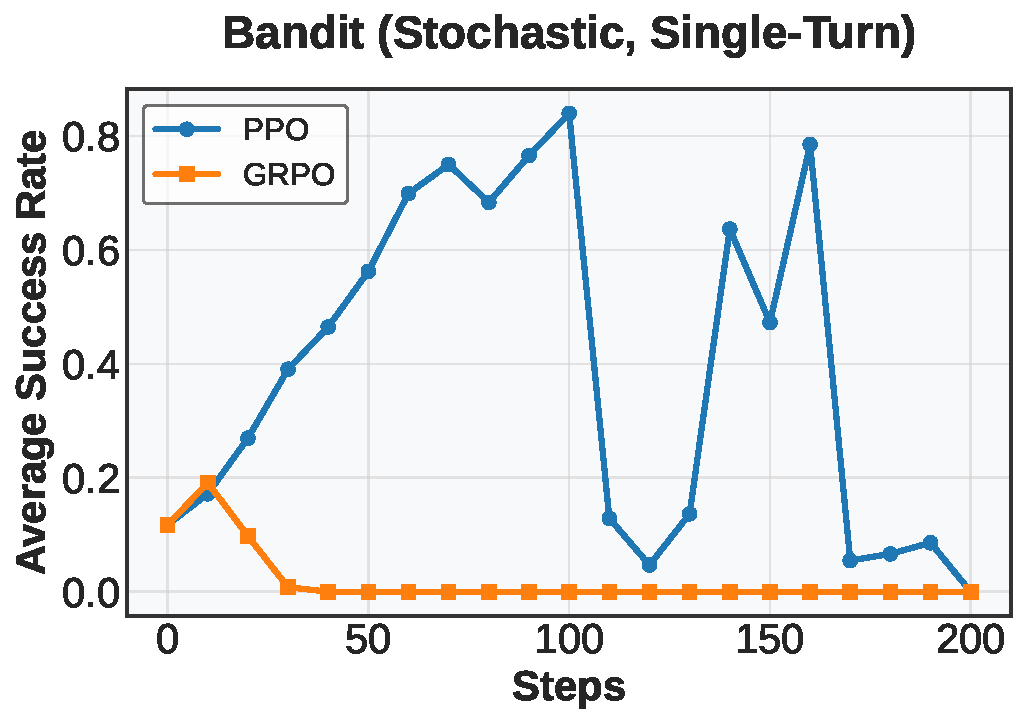
\includegraphics[width=0.32\linewidth]{figures/0_bandit_performance.pdf}
%   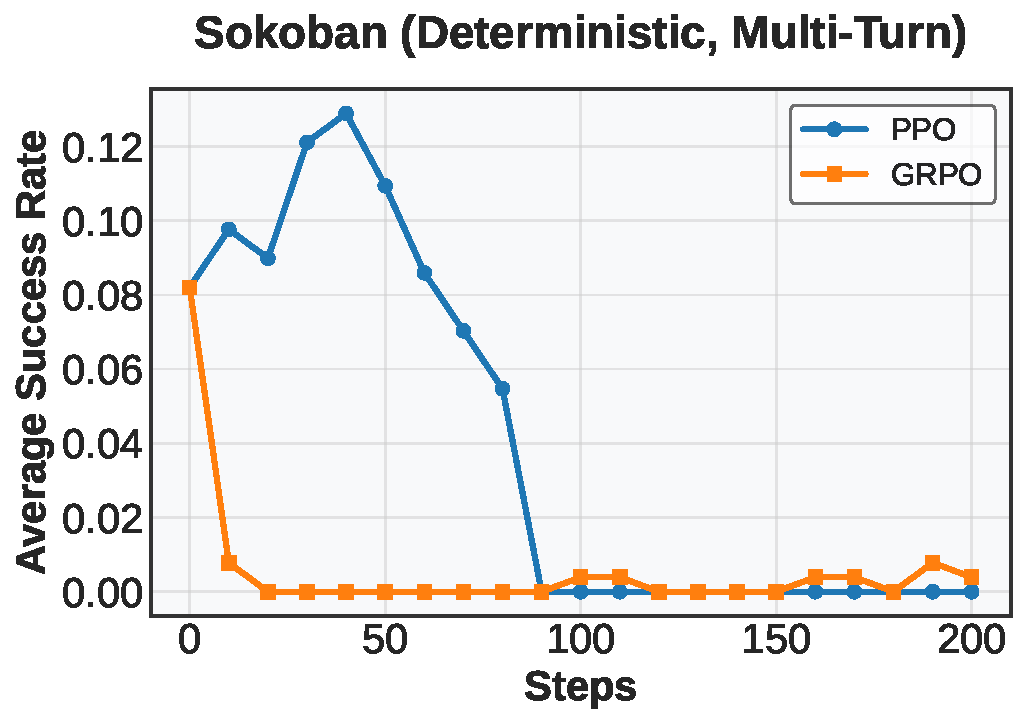
\includegraphics[width=0.32\linewidth]{figures/0_sokoban_performance.pdf}
%   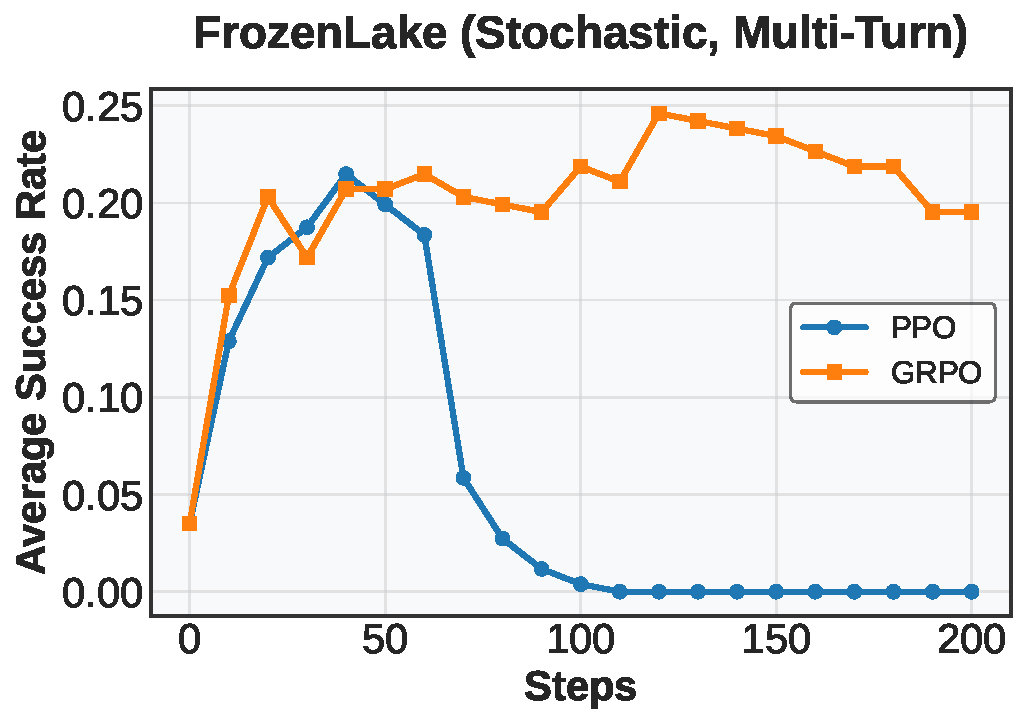
\includegraphics[width=0.32\linewidth]{figures/0_frozenlake_performance.pdf}
%     \caption{
%     \textbf{Baseline StarPO performance across environments.}
%     All StarPO runs initially improve but eventually collapse in multi-turn agent settings. PPO variant shows better training stability compared to the GRPO variant, especially in Bandit and Sokoban, indicating that critic-based methods better resist early-stage degradation under long-horizon dynamics.
%     }
%   \label{fig:task_performance}
% \end{figure}
\begin{figure}[t]
  \centering
  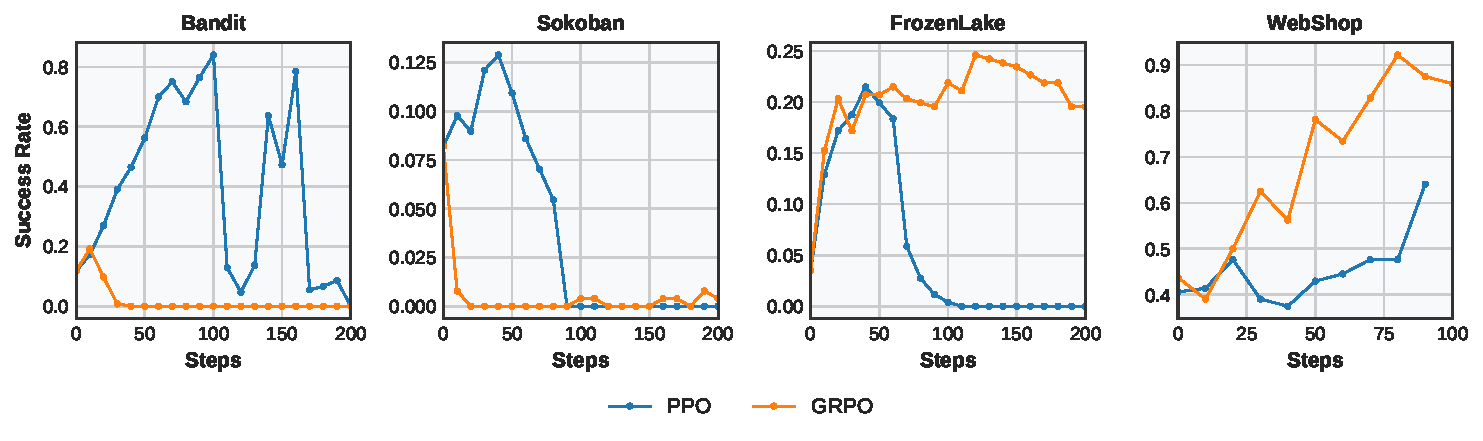
\includegraphics[width=\linewidth]{figures/ppo_vs_grpo.pdf}
    \caption{
    \textbf{Baseline StarPO performance across environments.}
     Symbolic tasks like Bandit and Sokoban lead to collapse while real-world WebShop starts high and improves fast. 
     PPO is stronger in Bandit and Sokoban to provide more stable token-level reward signal, while GRPO is stronger in Frozen Lake whose randomness makes the state value hard to estimate, and WebShop whose strong initial performance lessens the need for a critic to stabilize gradients.
    }
  \label{fig:task_performance}
  \vspace{-5pt}
\end{figure}


\newcolumntype{L}[1]{>{\raggedright\arraybackslash\small\ttfamily}p{#1}}


\begin{onebox}{Finding 1: Single-turn RL may not be directly adapted to Multi-turn agent RL}
Vanilla adaptations from single-turn methods like PPO and GRPO achieve early gains in agent settings but often collapse. A critic in PPO may delay instability, but would not prevent reasoning degradation, highlighting the need for specialized stabilization in agent settings.
\end{onebox}


To understand the causes of collapse, we compare early- and late-stage trajectories. In the Bandit task, early-stage trajectories exhibit diverse reasoning about symbolic meanings and expected rewards, while later-stage responses become repetitive and deterministic. This suggests that \textbf{RL training may have over-amplified inherent reasoning shortcuts}, reinforcing locally rewarded templates while suppressing exploration. 
We refer to this failure mode as an “\textbf{Echo Trap}”, which is similar to the findings in~\citet{recursivelygenerated}, where the model repeatedly reuses memorized reasoning paths when trained on self-generated trajectories, leading to a collapse in diversity and long-term performance degradation. Examples are in Appendix~\ref{app:echotrap}.

\begin{onebox}{Finding 2: Model collapse in agent RL is reflected as "Echo Trap" over training}
We find that early-stage agent respond with diverse symbolic reasoning, but collapse into deterministic, repetitive templates after training. Models converge to fixed phrasing, indicating that RL may reinforce superficial patterns instead of general reasoning and forms an "Echo Trap" that hinders long-term generalization.
\end{onebox}



To detect collapse, we monitor two key metrics: (1) \textbf{Average Reward}, where a plateau or drop signals degraded task performance, and (2) \textbf{Gradient Norm}, where spikes suggest unstable updates. To identify early signs, we also track rollout-level signals: (1) \textbf{Reward Standard Deviation}, indicating whether the policy is producing diverse outcomes or collapsing into repetitive behavior, and (2) \textbf{Output Entropy}, which indicates how deterministic the model’s predictions are.


% To determine whether collapse has already occurred, we track two metrics: (1) \textbf{Average Reward} whose plateau or drop identifies degraded task-solving ability, (2) \textbf{Gradient Norm} that measures update magnitude, with its spikes indicate that small updates are triggering large changes, typically a sign of training instability and collapse.


% To identify early signs of collapse, we further analyze rollout-level statistical signals that reflect behavioral redundancy and policy instability. Specifically, we examine two early indicators:
% (1) \textbf{Reward Standard Deviation} that measures whether rollouts under the same task instance lead to diverse outcomes or has collapsed into repetitive patterns with similar returns, (2) \textbf{Output Entropy} that captures the uncertainty of the model’s output, whose sharp drop implies the policy is becoming overconfident and converging to narrow reasoning paths. 

\begin{figure}[t]
  \centering
  % 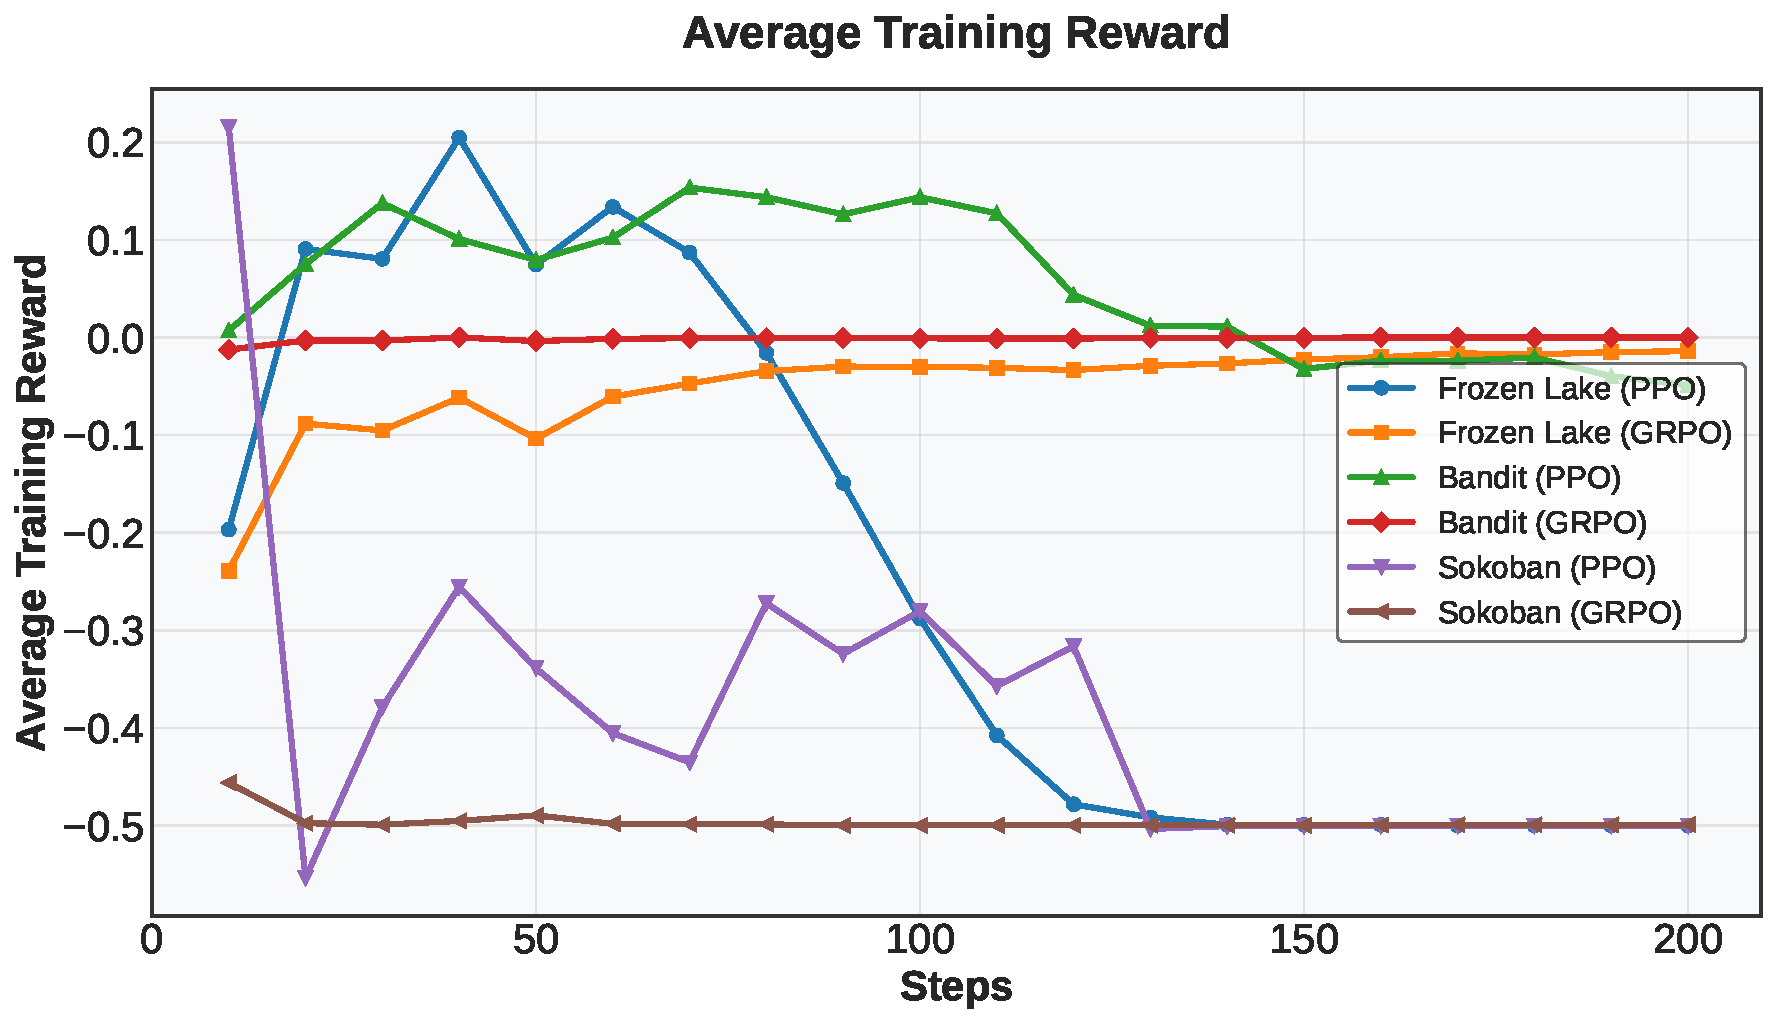
\includegraphics[width=0.48\textwidth]{figures/1_1_in_group_mean.pdf}
  % 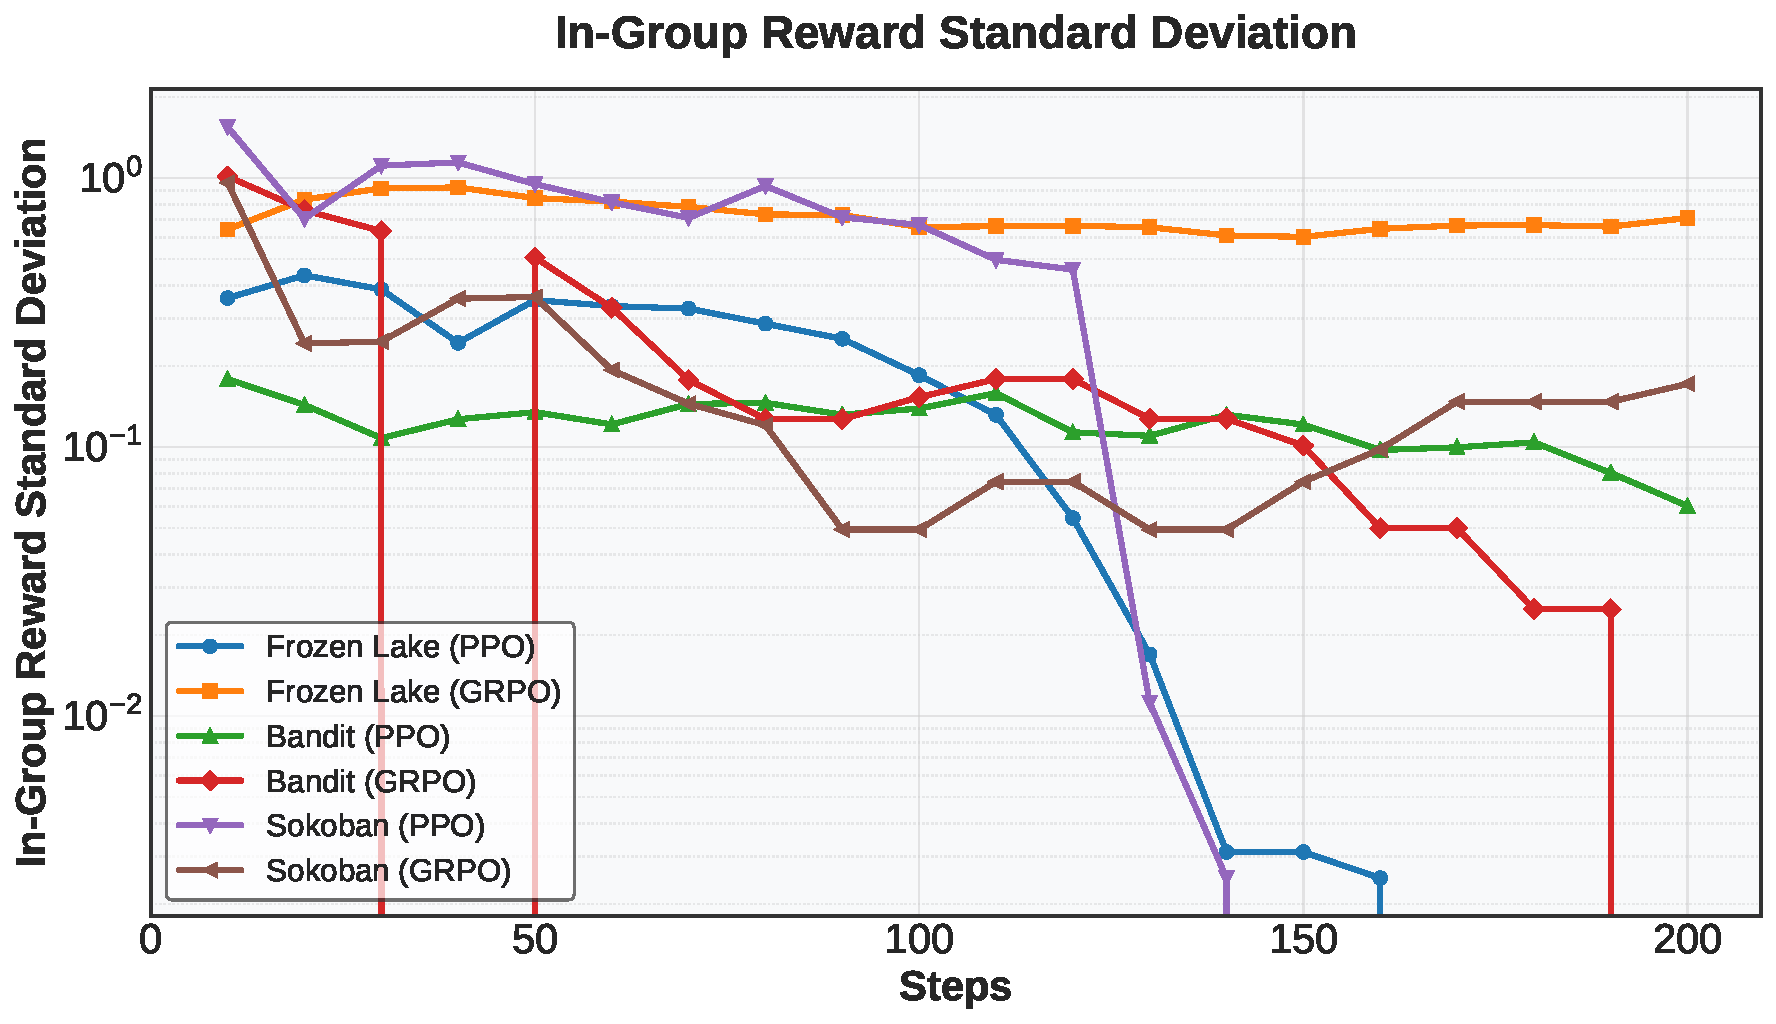
\includegraphics[width=0.48\textwidth]{figures/1_1_in_group_std.pdf}
  % 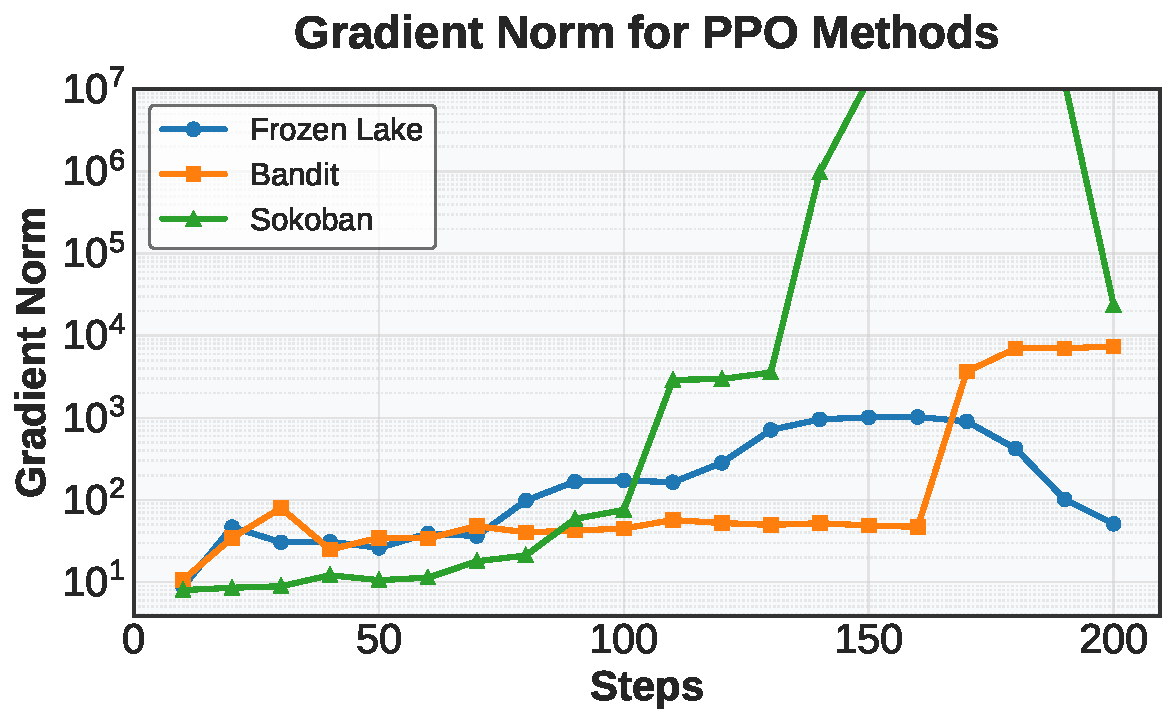
\includegraphics[width=0.24\textwidth]{figures/1_2_grad_norm_ppo.pdf}
  % 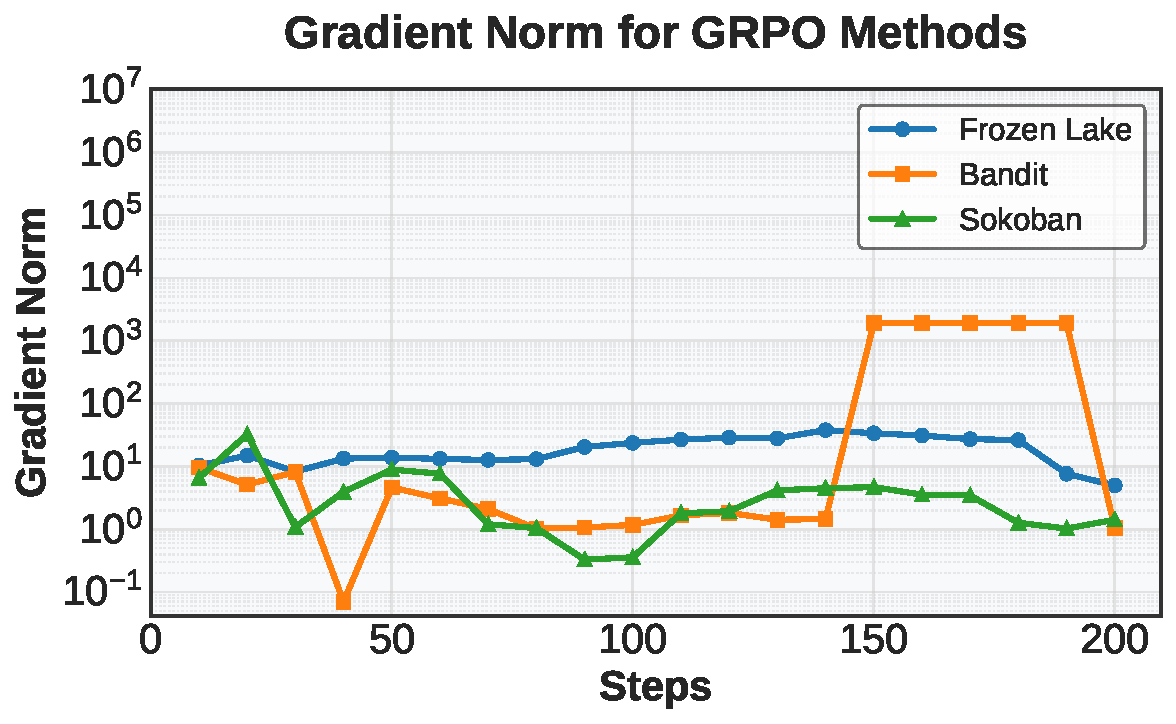
\includegraphics[width=0.24\textwidth]{figures/1_2_grad_norm_grpo.pdf}
  % 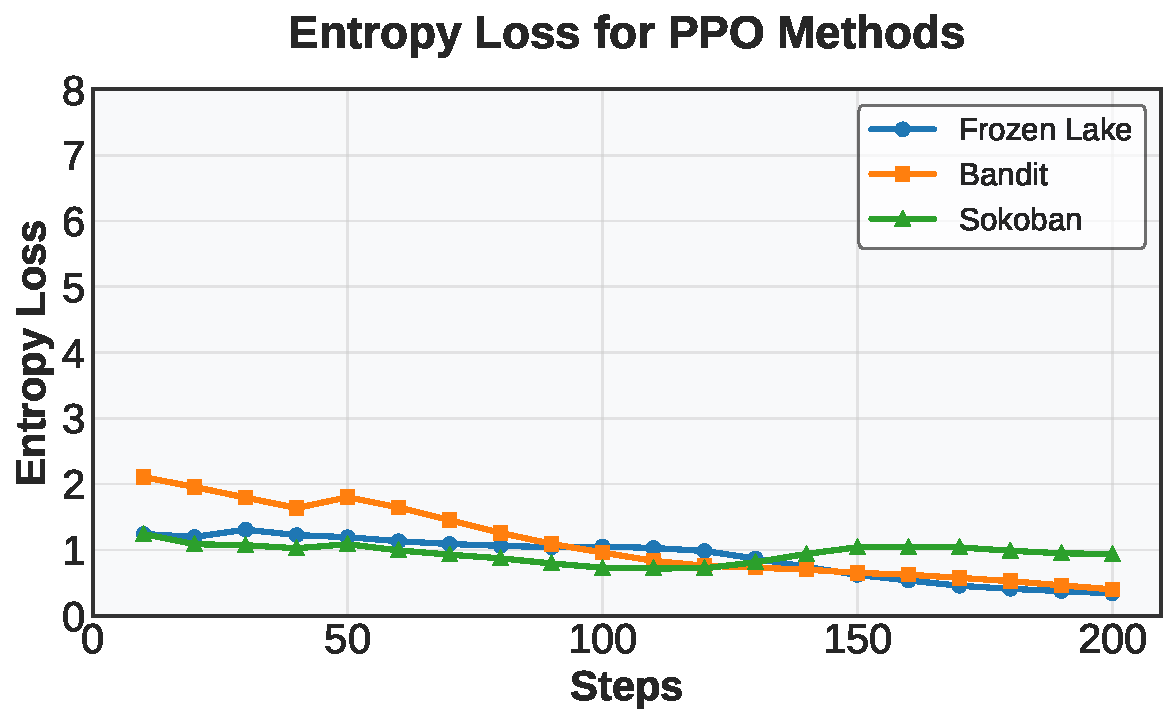
\includegraphics[width=0.24\textwidth]{figures/1_2_entropy_loss_ppo.pdf}
  % 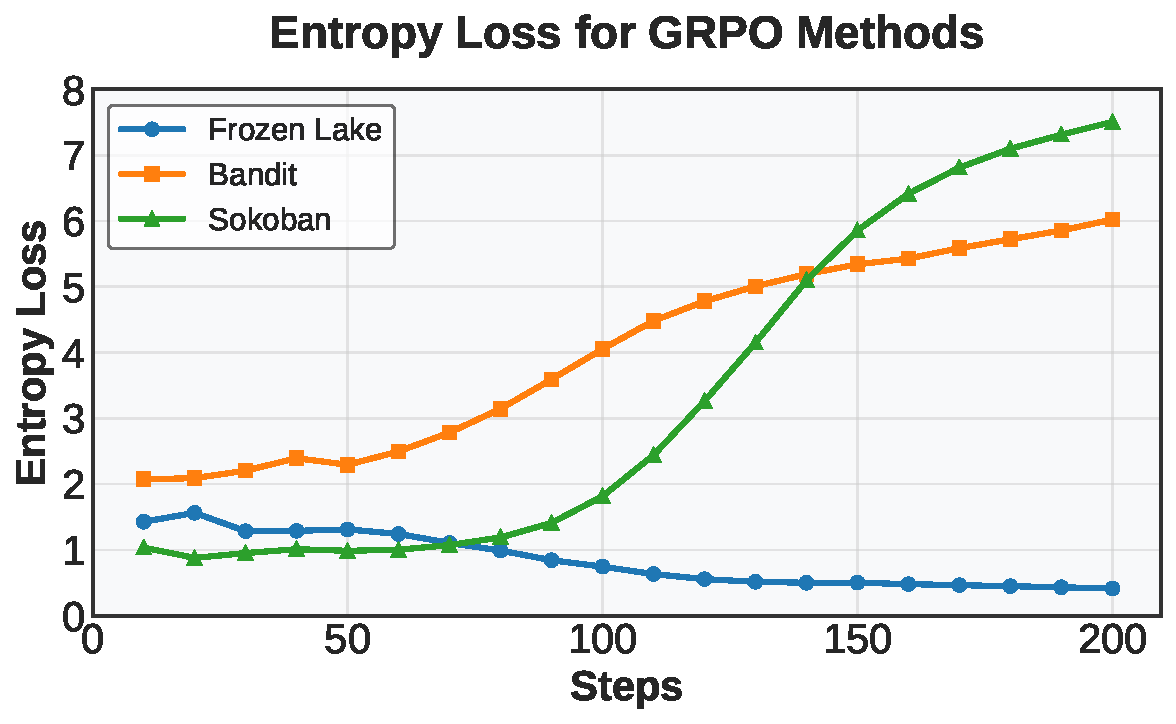
\includegraphics[width=0.24\textwidth]{figures/1_2_entropy_loss_grpo.pdf}
  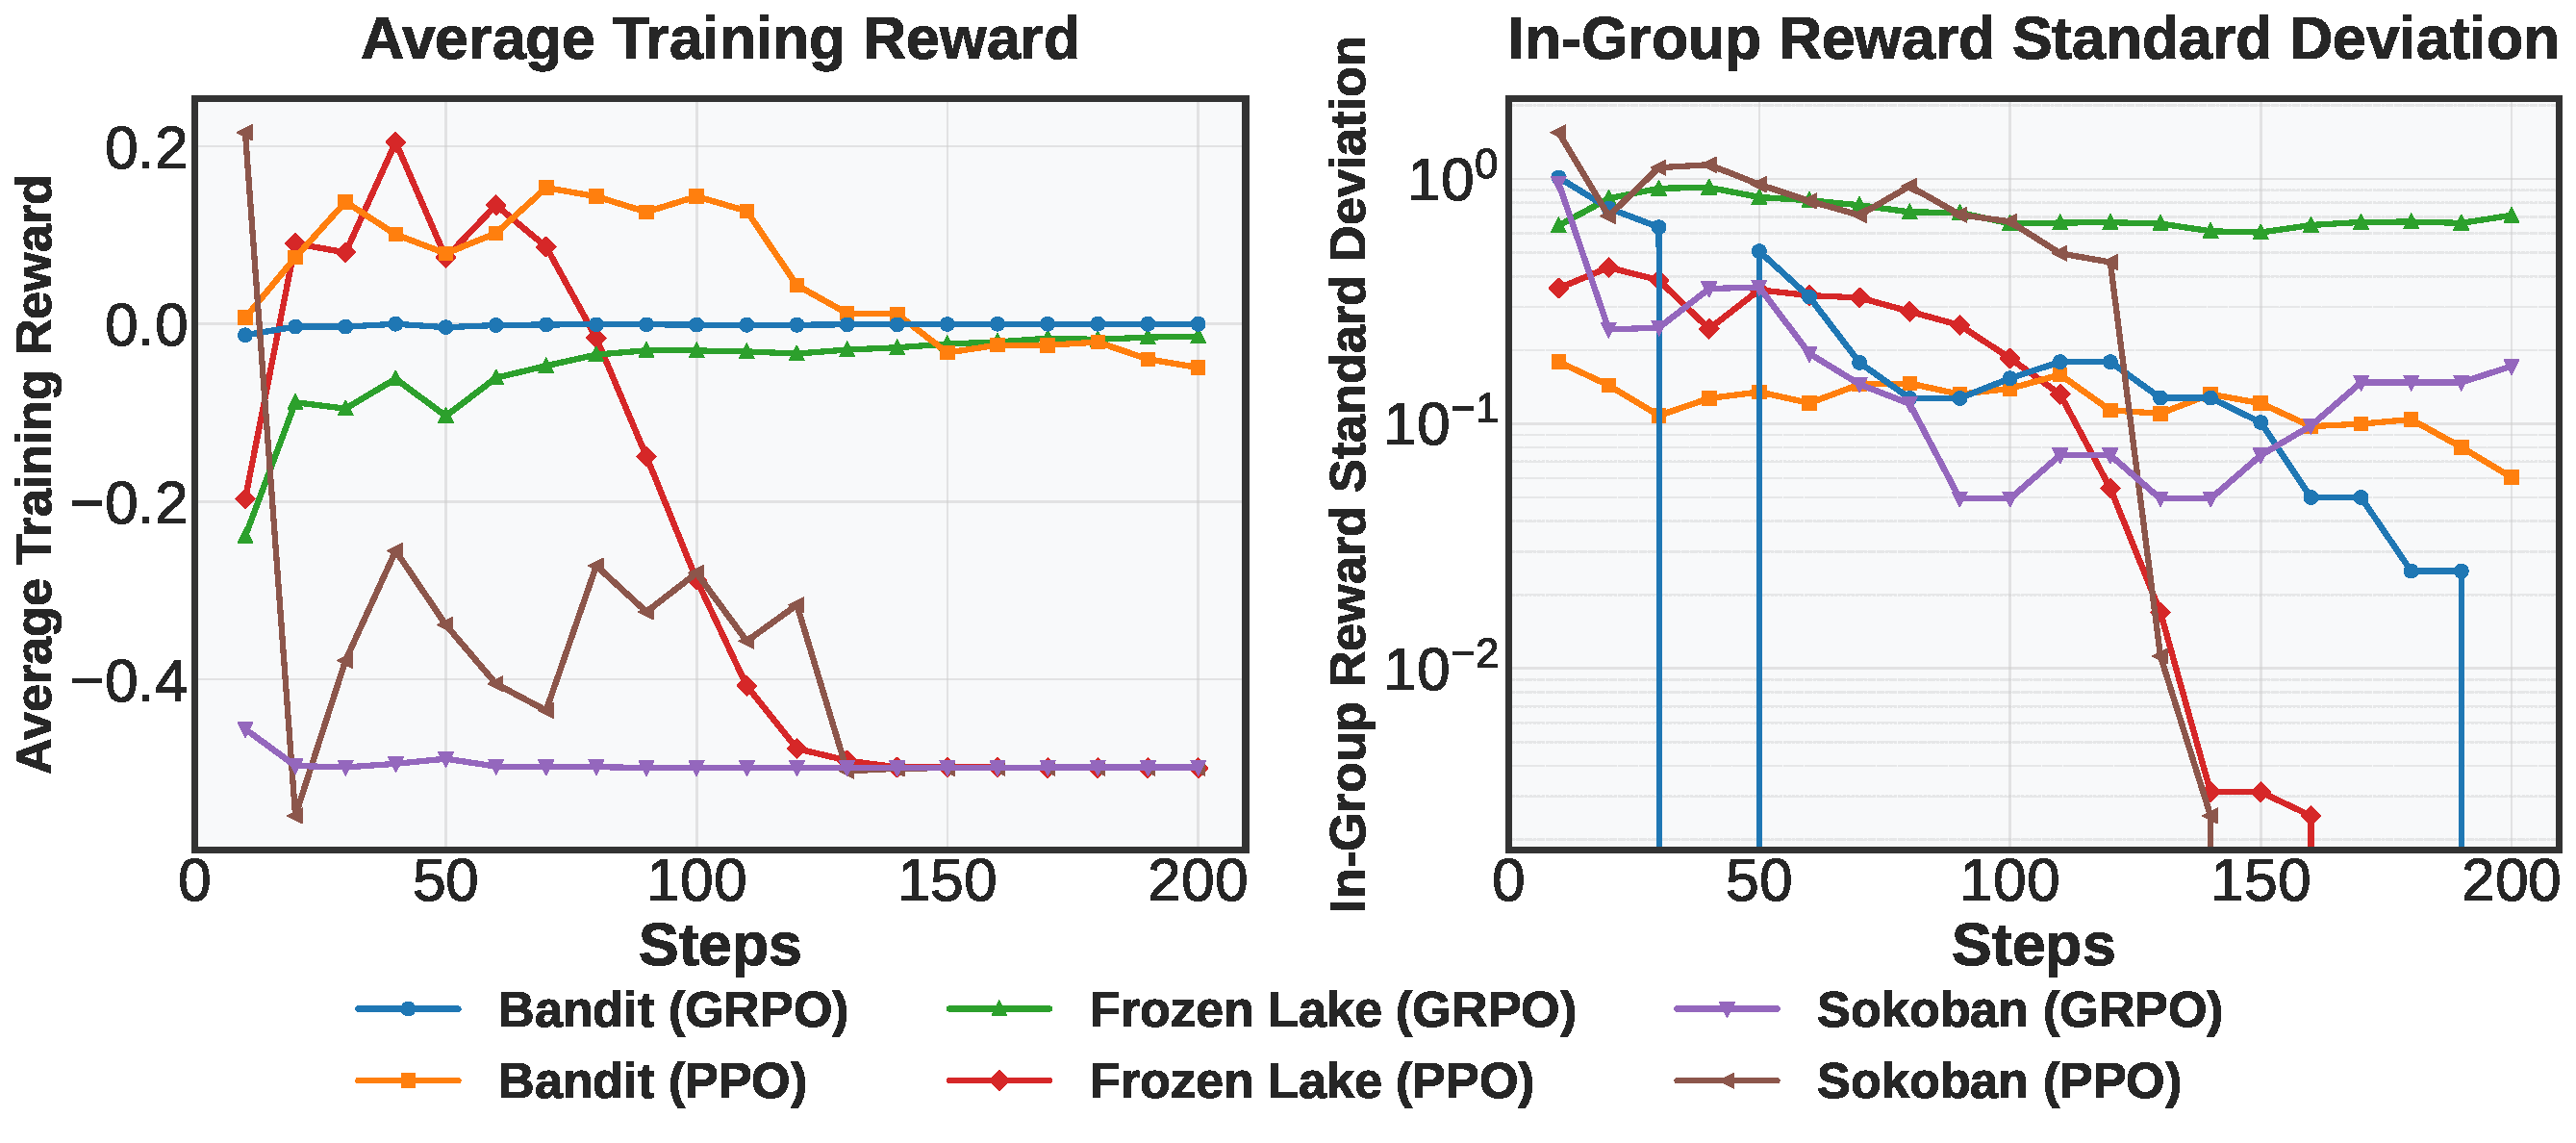
\includegraphics[width=0.7\textwidth]{figures/figures_combined/figure6_1_collapse_indicators.pdf}
  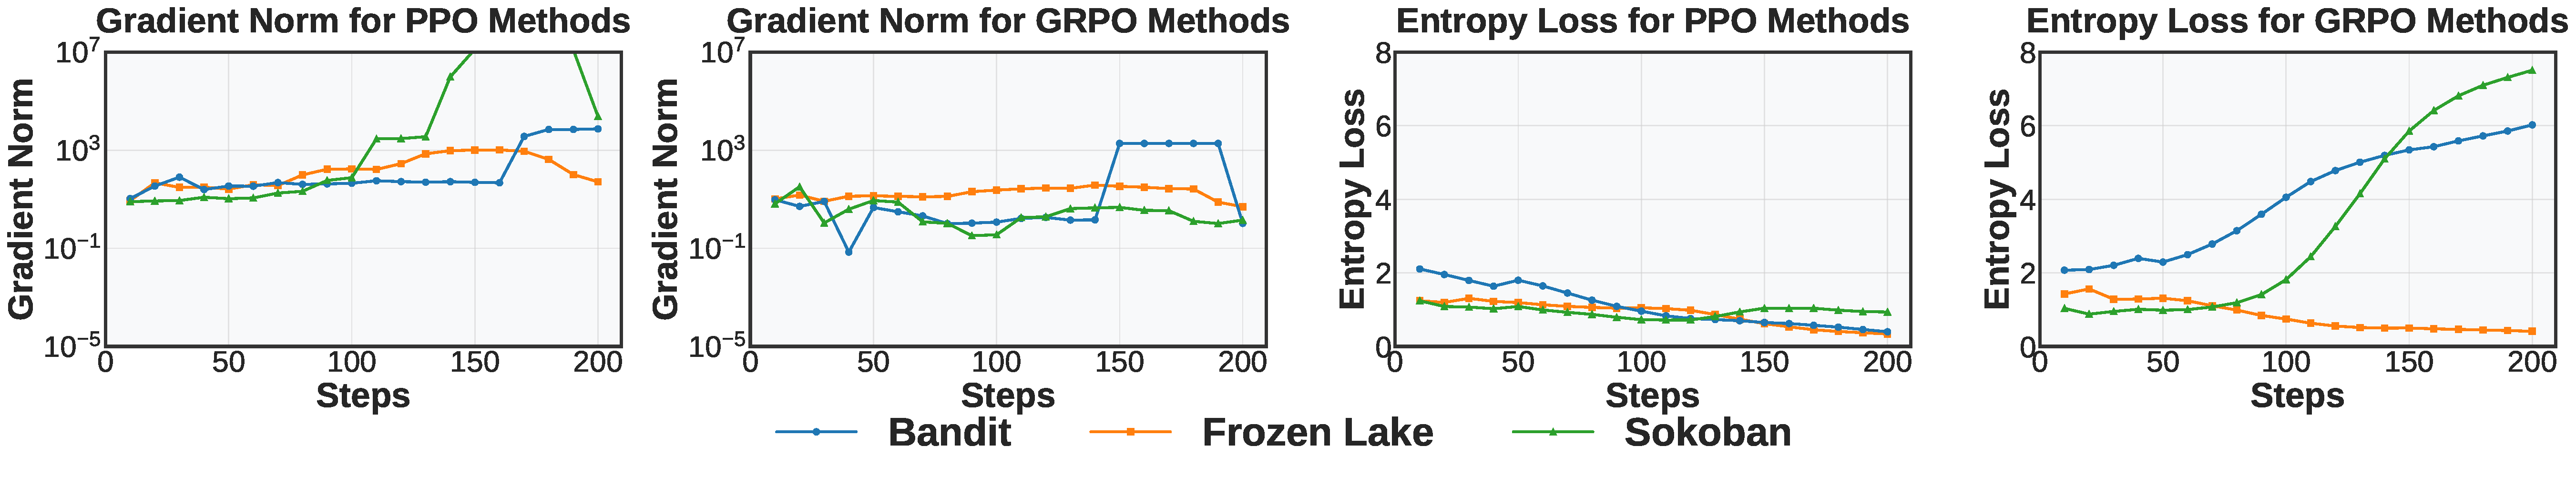
\includegraphics[width=\textwidth]{figures/figures_combined/figure6_2_collapse_indicators.pdf}
  \caption{
\textbf{Collapse indicators and early warning signals in multi-turn RL.}
Average reward and gradient norm (left-side plots) reflect collapse directly, and their plateaus and spikes confirm performance and training instability.
Reward standard deviation and entropy (right-side plots) often becomes unstable before reward degrades, serving as early warning signals. 
}
  \label{fig:collapse_metrics}
  \vspace{-5pt}
\end{figure}


% Figure~\ref{fig:collapse_metrics} summarizes these dynamics across tasks and optimization methods. From the results, we summarize key conclusions regarding \textbf{how model collapse happens}:
% \vspace{-5pt}
% \begin{itemize}
%     \item \textbf{Reward Std is a strong predictor for model collapse in agent RL.} For FrozenLake-PPO, reward mean collapses at 90 steps, but std drops sharply as early as 40 when the reward mean reaches the peak—serving as an early warning. In Bandit-PPO, std reaches its lowest point around 70 steps, just as reward peaks at 120. In Sokoban-PPO, std and mean collapse almost simultaneously around step 10.
%     \item \textbf{Gradient norm spikes mark the point of complete collapse.} After gradient norm spikes in PPO appear at 170 (Bandit), 110 (Sokoban), and 90 (FrozenLake), it basically means even small updates cause destabilizing shifts, rendering the model unable to recover after acute update steps.
%     
% \end{itemize}
% \vspace{-5pt}

Figure~\ref{fig:collapse_metrics} summarizes these dynamics across tasks and optimization methods. From the results, we draw the following conclusions regarding \textbf{how model collapse emerges in multi-turn agent RL}:
\vspace{-5pt}
\begin{itemize}[left=2pt, itemsep=2pt, topsep=4pt]
    \item \textbf{Reward standard deviation is an early indicator of convergence.} In FrozenLake-PPO, std drops sharply at step 40, well before reward mean collapses at step 90 while performance is near-optimal. In Bandit-PPO, std bottoms out around step 70, preceding the reward peak at step 120. In Sokoban-PPO, std and mean collapse together near step 10, suggesting early saturation. 

    
    \item \textbf{Gradient norm spikes indicate irreversible collapse.} Once gradient norm spikes emerge, e.g., at step 170 (Bandit), 110 (Sokoban), and 90 (FrozenLake), even small parameter updates could induce drastic loss shifts, after which recovery becomes unlikely.
    
    \item  \textbf{Entropy should follow a stable decay trend during effective learning}. This can be seen from FrozenLake-GRPO. Rapid entropy increases or erratic changes often correlate with collapsed reasoning behavior, such as GRPO on Bandit and Sokoban.
\end{itemize}
\vspace{-9pt}

\begin{onebox}{Finding 3: Collapse follows similar dynamics and can be anticipated by indicators}
\textbf{Reward standard deviation} and \textbf{entropy} often fluctuate before performance degrades, while \textbf{gradient norm} spikes typically mark the point of irreversible collapse. These metrics provide early indicators and motivate the need for stabilization strategies.
\end{onebox}
These patterns confirm that multi-turn RL introduces unique challenges that single-turn RL methods fail to handle. In response, we introduce \textbf{StarPO-S}, a stabilized variant that targets sampling quality, gradient stability, and exploration regularization to avoid premature collapse.




\subsection{StarPO-S: Stabilize Multi-turn RL with Instance Filtering and Gradient Shaping}

To address the instability of multi-turn reinforcement learning, we introduce \textbf{StarPO-S}, a stabilized variant of StarPO that incorporates three key modifications aimed at improving training robustness and efficiency. Building on the insight that declining reward standard deviation often precedes collapse, we investigate the following question: \textit{should agents be trained more intensively on task instances where their behavior is more uncertain with higher reward variability?} 

We hypothesize that the most effective training samples are those where the agent \textbf{exhibits outcome uncertainty}—avoiding both trivial task instances and overly difficult ones. This intuition is rooted in principles of Active Learning~\citep{activelearning}, where uncertain examples are the most informative ones models should learn from. We define trajectory-level outcome uncertainty $U$ for policy $\pi_\theta$ on a given agent task instance (initial state $s_0$ in an MDP $\mathcal{M} = \{S, A, P\}$) as:
\begin{equation}
\text{U}(\pi_{\theta}, \mathcal{M}, s_0) = \text{Std}_{\tau \sim \pi_\theta(\cdot | s_0)}\left[R(\tau)\right].
\end{equation}
During training, we sort prompts based on the standard deviation of reward obtained from repeated rollouts and \textbf{retain only the top $p$\% highly-uncertain prompts} at each training step. Figure~\ref{fig:filtering_starpos} shows the effect of varying $p$ in PPO and GRPO under StarPO-S. We further validate the effect of uncertainty-based filtering in Appendix~\ref{app:std}.


In PPO runs (Figure~\ref{fig:filtering_starpos}, left), filtering low-variability rollouts significantly delays collapse: retaining 75\% of rollouts extends stability in FrozenLake from 100 to 140 steps, while 50\% avoids collapse entirely. GRPO remains less stable due to its critic-free design but still benefits modestly. Filtering also improves efficiency (Figure~\ref{fig:filtering_starpos}, right). We adopt 25\% as the default for StarPO-S. However, we note that this aggressive value may not be optimal for all scenarios.
Tasks like Sokoban and FrozenLake respond well to aggressive filtering, potentially due to their relatively repetitive reasoning patterns and under-representation in pretraining, which make them tend to collapse when similar trajectories dominate the batch. We further present larger model (72B), together with frontier model such as GPT-4o and Qwen-2.5-72B, in Appendix~\ref{app:largermodelabaltion}, to better contextualize our model performance.

\begin{onebox}{Finding 4: Filtering low-variance trajectories improves stability and efficiency}
Training on high-variance prompts delays or eliminates collapse in multi-turn RL. StarPO-S improves performance and reduces update steps by discarding low-information rollouts, especially under PPO. This aligns with active learning principles, where uncertain examples offer the most informative learning signals.
\end{onebox}

In addition to uncertainty-based filtering, we adopt two gradient shaping techniques inspired by DAPO~\citep{yu2025DAPO} designed for single-turn RL: \textbf{KL Term Removal} and \textbf{Clip-Higher} (Asymmetric Clipping). We extend and evaluate them in the multi-turn agent setting, and find both methods boost the success rate and extend stable training phases, showing how multi-turn RL benefits from more flexible gradient shaping. Design details and performance ablation is in Appendix~\ref{app:largermodelabaltion}.

\begin{figure}[t]
  \centering
  % 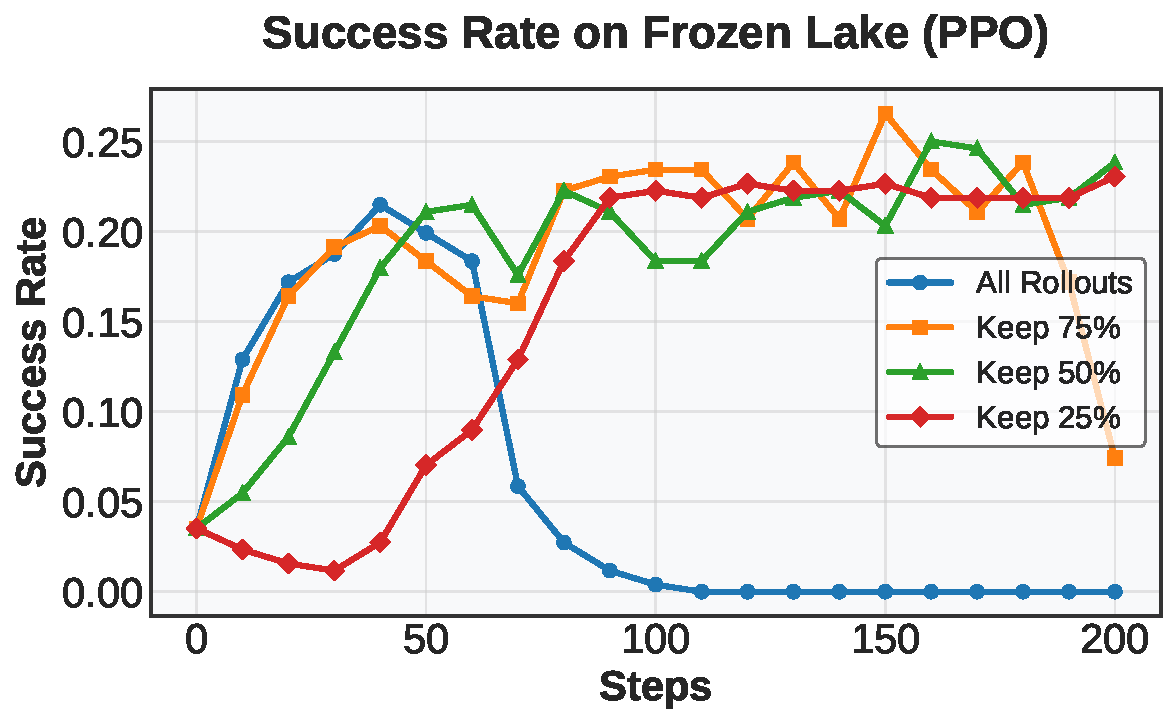
\includegraphics[width=0.32\textwidth]{figures/2_frozen_lake_filter_ppo.pdf}
  % 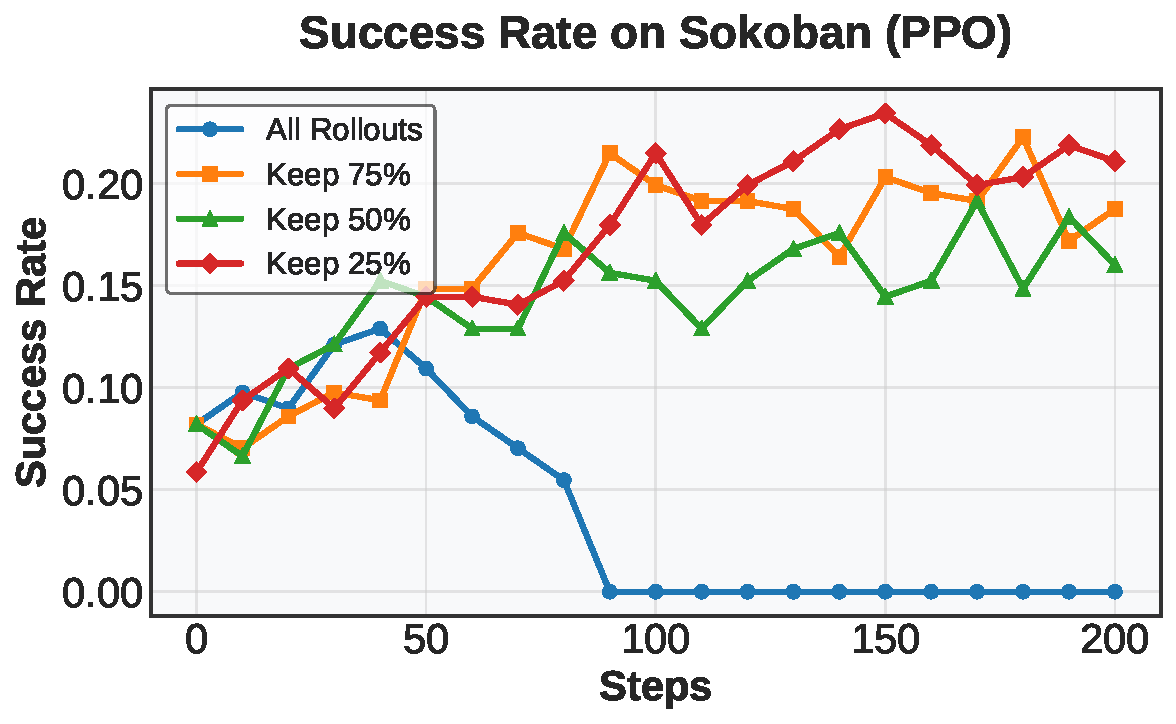
\includegraphics[width=0.32\textwidth]{figures/2_sokoban_filter_ppo.pdf}
  % 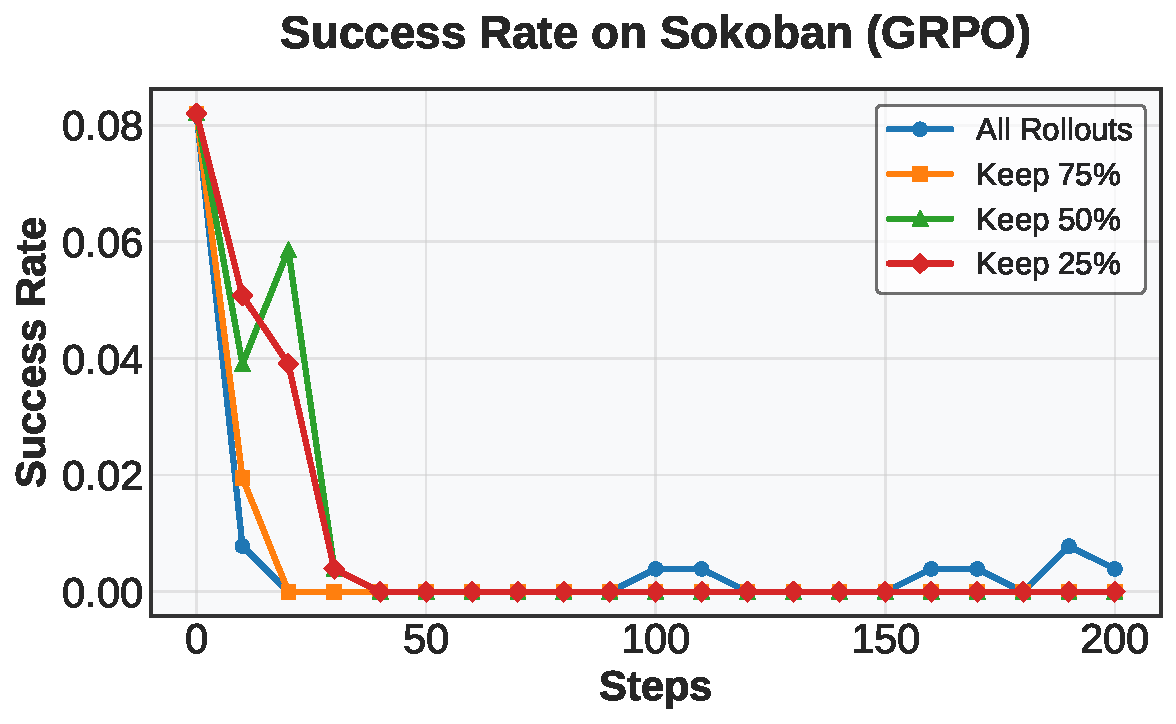
\includegraphics[width=0.32\textwidth]{figures/2_sokoban_filter_grpo.pdf}
  % 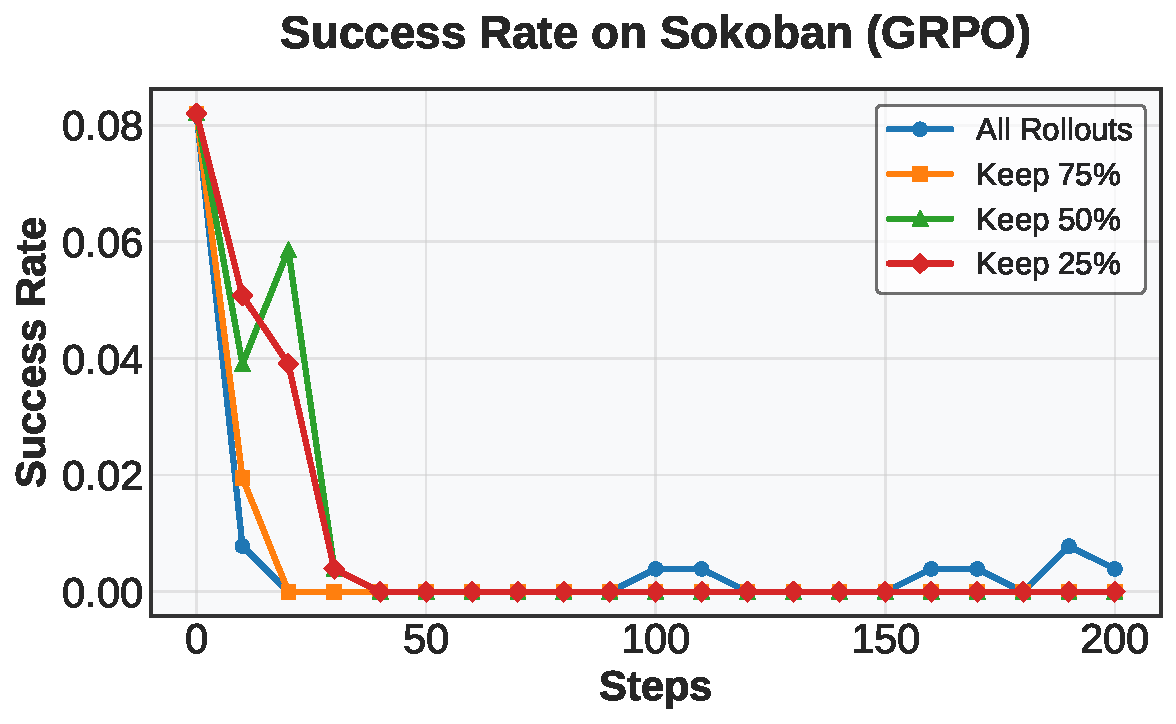
\includegraphics[width=0.24\textwidth]{figures/2_sokoban_filter_grpo.pdf}
  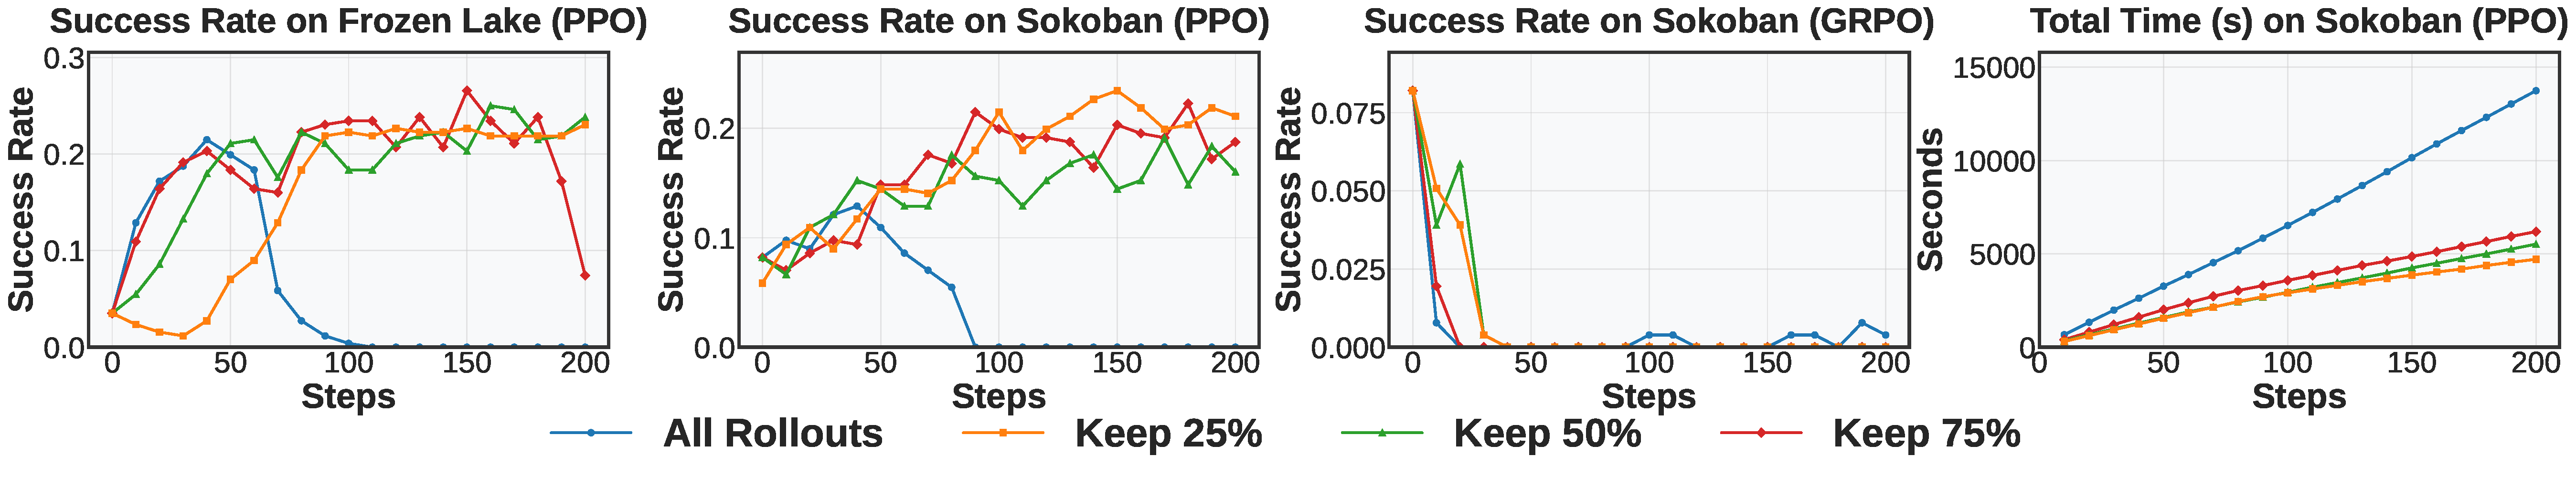
\includegraphics[width=\textwidth]{figures/figures_combined/figure7_effect_uncertainty.pdf}
  \caption{\textbf{Effect of uncertainty-based filtering on multi-turn RL stability.} Filtering out low-variability trajectories reduces collapse risk and improves success rate. On PPO variants, collapse is largely mitigated when more than half of the trajectories are filtered. Training time is reduced.}
  \label{fig:filtering_starpos}
  \vspace{-5pt}
\end{figure}


\noindent\textbf{Overall Comparison.}~~
    We compare StarPO-S with vanilla StarPO across three tasks in Figure~\ref{fig:starpos_summary}. StarPO-S consistently delays collapse and enhances final task performance. We attribute these gains to more selective training data (via uncertainty filtering), more balanced optimization signals (via KL removal and decoupled clipping), reducing narrowed reasoning modes. In the appendix~\ref{app:largermodelabaltion}, we further discuss about other variants that may stablize training and enhance performance, such as selective response mask and Bi-level Gegenal Advantage Estimation (GAE)~\cite{vagen}.

\begin{figure}[t]
  \centering
  % 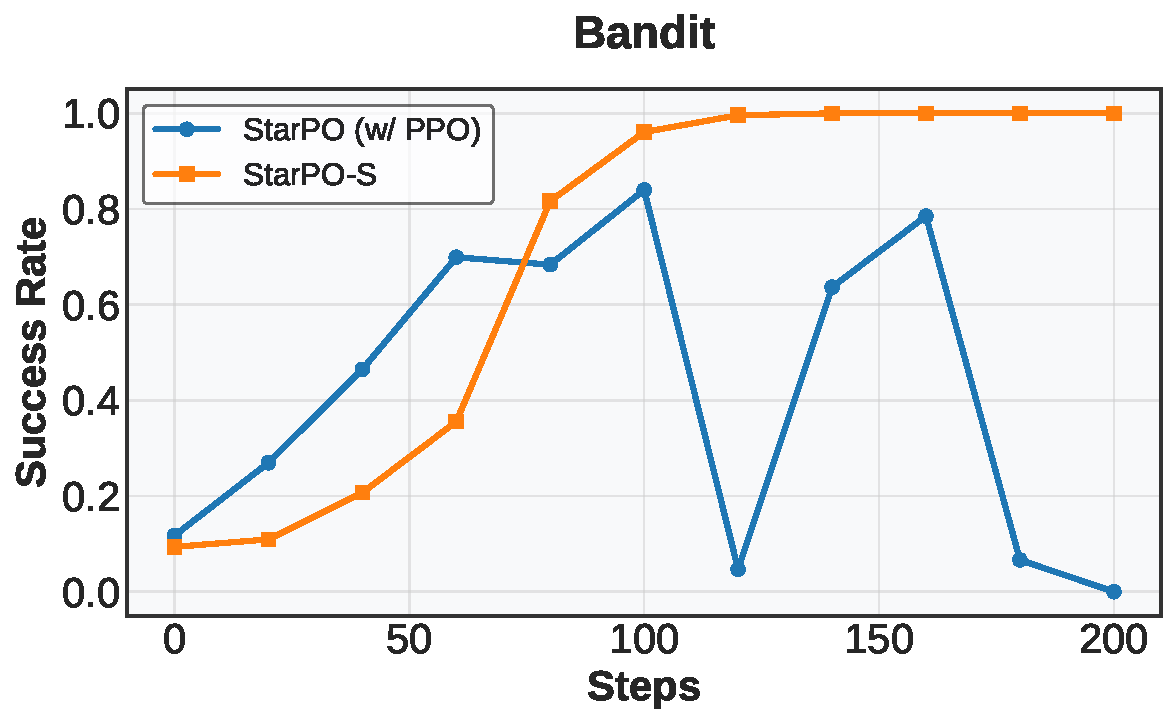
\includegraphics[width=0.32\textwidth]{figures/4_bandit_compare_ppo_starpo_s.pdf}
  % 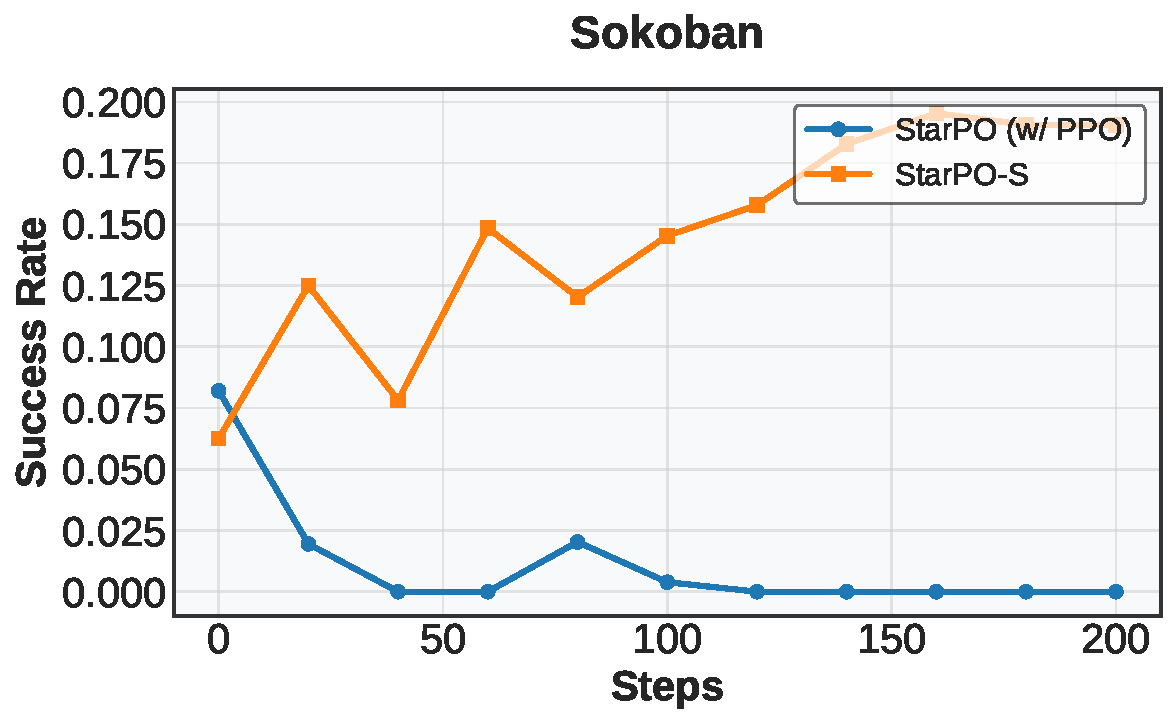
\includegraphics[width=0.32\textwidth]{figures/4_sokoban_compare_ppo_starpo_s.pdf}
  % 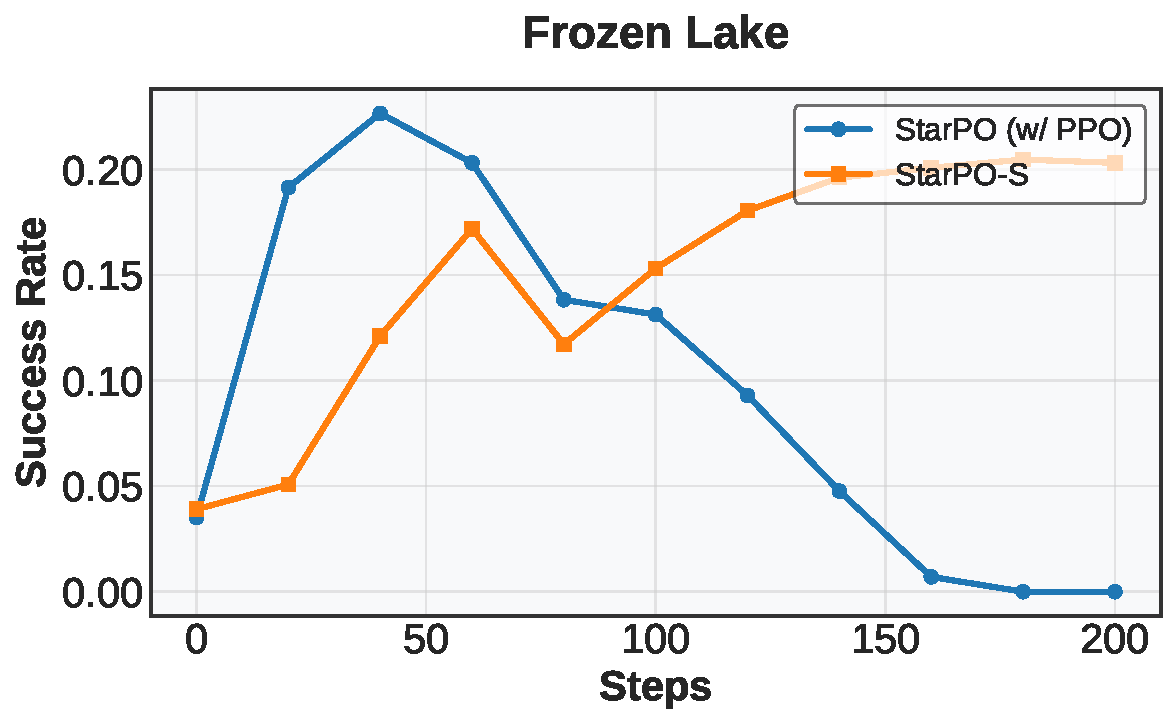
\includegraphics[width=0.32\textwidth]{figures/4_frozenlake_compare_ppo_starpo_s.pdf}
  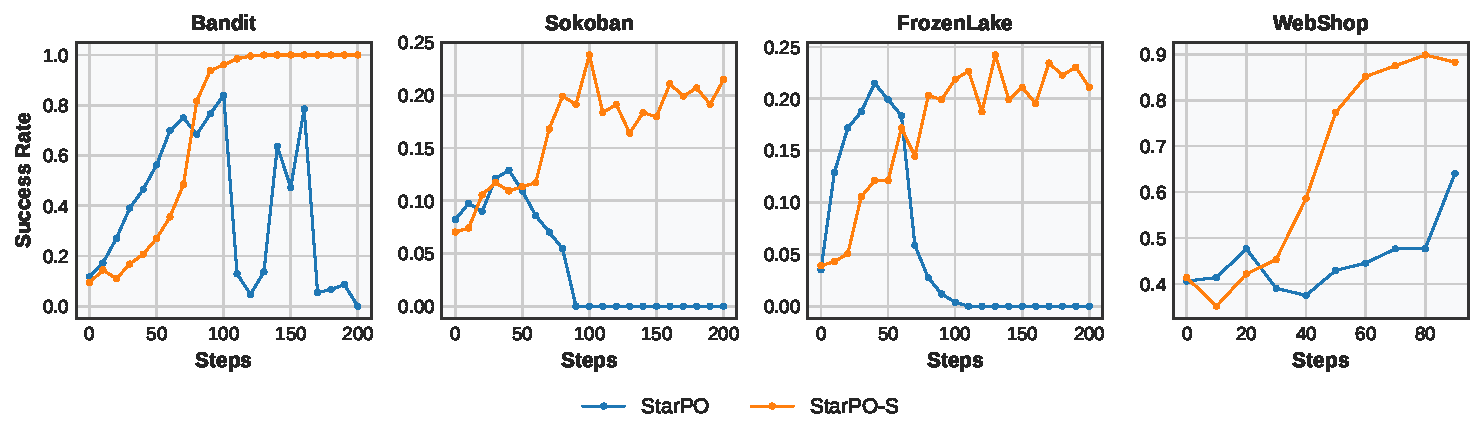
\includegraphics[width=\textwidth]{figures/starpo_vs_s.pdf}
  \caption{\textbf{StarPO-S improves stability and final performance across tasks.} Compared to vanilla StarPO, StarPO-S reliefs collapse in all four tasks and could achieves higher success rates. }
  \label{fig:starpos_summary}
  \vspace{-9pt}
\end{figure}

% In addition to filtering, we incorporate two enhancements adapted from DAPO~\citep{yu2025DAPO} for stabilizing single-turn RL, and evaluate their effect in multi-turn settings:

% \begin{itemize}
%     \item \textbf{KL Removal:} We remove the KL divergence penalty from PPO's loss function, relying solely on policy loss and entropy bonus to shape the update.
%     \item \textbf{Clip-High (Decoupled Clipping):} We apply asymmetric clipping ranges in PPO: a higher upper bound (e.g., $\epsilon_\text{high} = 0.4$) than the lower bound ($\epsilon_\text{low} = 0.1$), allowing larger gradient updates on high-reward trajectories while suppressing punishment for wrong but low-reward ones.
% \end{itemize}

% \begin{figure}[H]
%   \centering
%   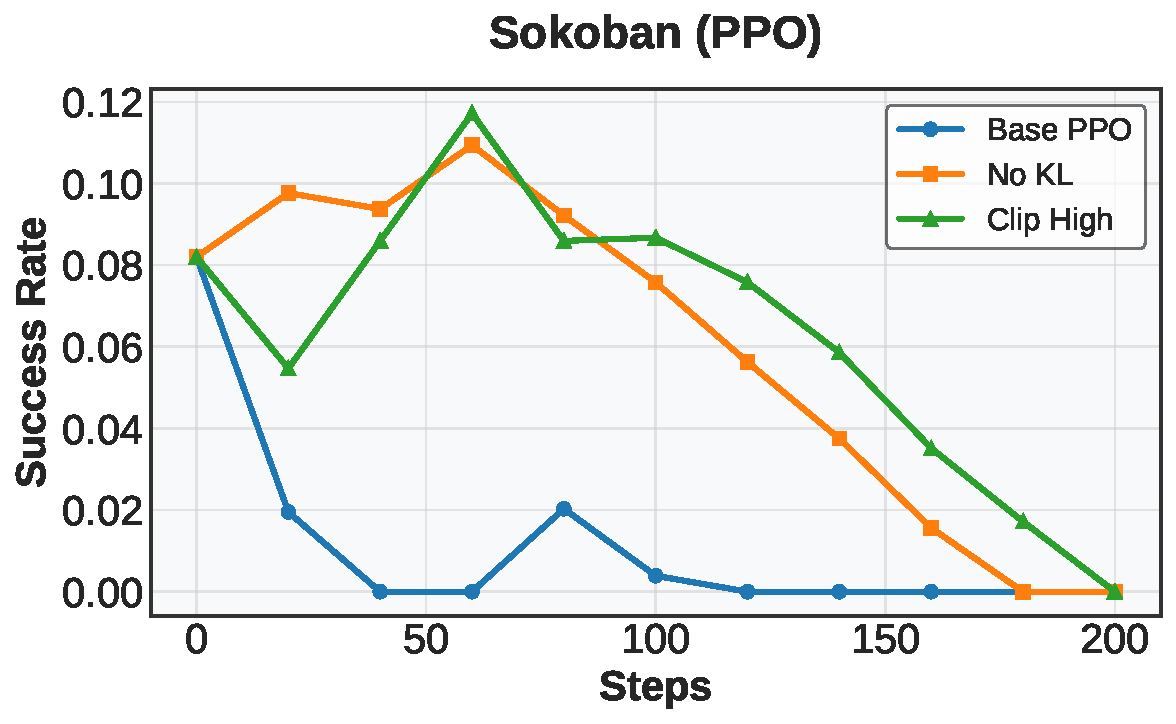
\includegraphics[width=0.48\textwidth]{figures/3_sokoban_comparetrick_ppo.pdf}
%   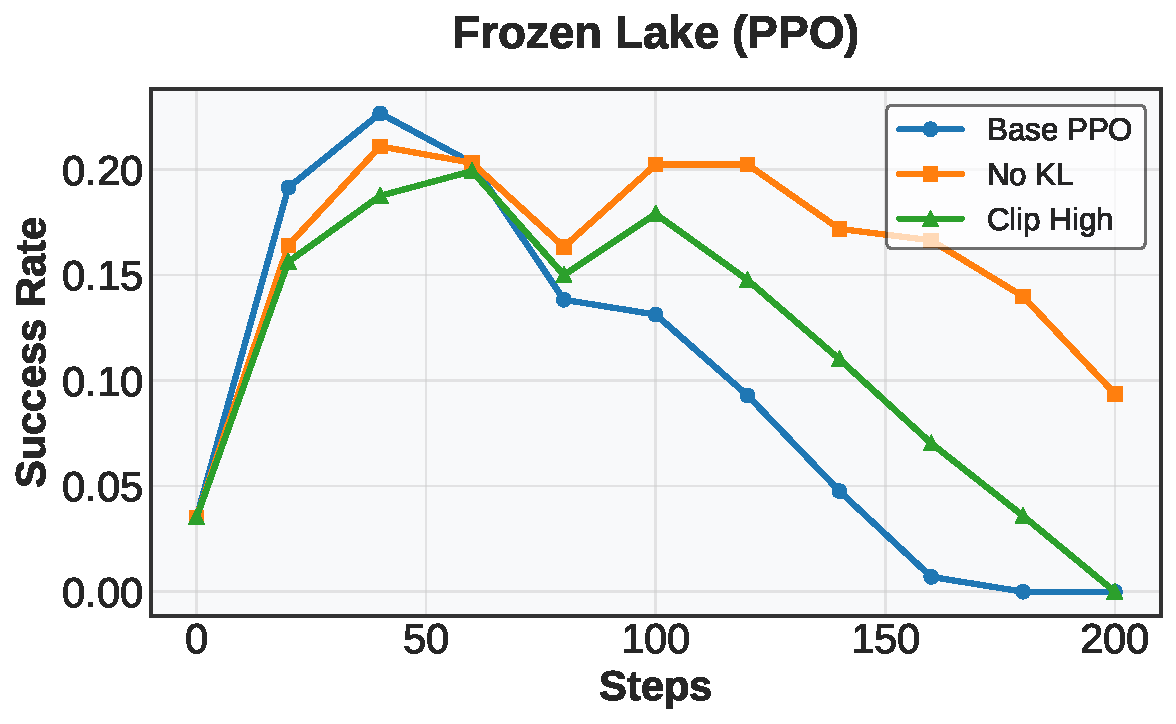
\includegraphics[width=0.48\textwidth]{figures/3_frozenlake_comparetrick_ppo.pdf}
%   \caption{Effect of KL removal and asymmetric clipping (ClipHigh) in PPO. Both improve peak performance and delay collapse.}
%   \label{fig:trick_results}
% \end{figure}

% As seen in Figure~\ref{fig:trick_results}, both methods increase the peak success rate and extend training stability in PPO. This supports the idea that multi-turn RL agents benefit from more selective gradient shaping—focusing on amplifying effective reasoning paths rather than aggressively penalizing noisy ones.





\subsection{Generating Useful Trajectories for RL Training}
\label{sec:rollout}
Effective RL training depends heavily on trajectory quality. We study three key rollout dimensions—\textit{task diversity}, \textit{interaction granularity}, and \textit{rollout frequency}—by training on vanilla Sokoban and evaluating on other tasks including SokobanNewVocab, LargeSokoban, and FrozenLake Task, which we detail in Appendix~\ref{app:generalization-task}.

\noindent\textbf{Higher task diversity with response comparison improves generalization.}~~
Task diversity refers to the number of distinct prompts used for each rollout-update cycle. With a fixed batch size, it trades off against the number of responses per prompt. 
In our experiments (Table~\ref{tab:diversity}), we vary this trade-off and find that higher task diversity—achieved by fewer responses per prompt (e.g., 4 per prompt)—consistently yields better generalization. This only holds when each prompt includes multiple rollouts, enabling the agent to contrast different outcomes under similar conditions.

\noindent\textbf{Allowing more action budgets enables planning, while overly long-horizon rollouts inject noise.}~~
We vary the number of actions allowed per turn in Table~\ref{tab:granularity}. Allowing up to 5 or 6 actions per turn yields the best performance, especially on complex environments like SokobanNewVocab and LargeSokoban. This setting provides enough room for planning while avoiding the chaos of overly long rollouts. Increasing the budget to 7 actions degrades performance, likely due to noisy transitions and diluted reward feedback.

\begin{table}[t]
  \centering
  \small
    \caption{\textbf{Effect of Task Diversity on Generalization Performance (\%).} Higher diversity with multiple responses yields the best performance (4 responses per prompt).}
  \begin{tabular}{lccc}
    \toprule
    \textbf{Response Per Prompt} & \textbf{SingleSokoban} & \textbf{SokobanNewVocab} & \textbf{FrozenLake} \\
    \midrule
    32   & 21.09\% & 20.22\% & 17.97\% \\
    16   & 20.31\% & 21.48\% & 19.53\% \\
    8  & 20.31\% & 19.53\% & 17.19\% \\
    4  & \textbf{20.70\%} & \textbf{25.39\%} & \textbf{21.48\%} \\
    2  & 19.92\% & 25.00\% & \textcolor{red}{12.50\%} \\
    1 & 19.53\% & 22.27\% & \textcolor{red}{12.50\%} \\
    \bottomrule
  \end{tabular}
    \vspace{-8pt}
  \label{tab:diversity}
\end{table}



\begin{table}[t]
  \centering
  \small
  \caption{\textbf{Performance across environments under different per-turn action budgets (\%).} 5--6 actions per turn yields best performance, balancing well for effective multi-step planning.}
  \begin{tabular}{lcccc}
    \toprule
    \textbf{Max Actions / Turn} & \textbf{Sokoban} & \textbf{SokobanNewVocab} & \textbf{LargeSokoban} & \textbf{FrozenLake} \\
    \midrule
    1 & 12.11\% & 13.67\% & 1.17\% & 11.72\% \\
    2 & 16.41\% & 21.09\% & 3.52\% & 18.36\% \\
    3 & 19.53\% & 19.53\% & 1.95\% & 20.88\% \\
    4 & 26.95\% & 26.95\% & 5.08\% & 20.70\% \\
    5 & 28.13\% & 25.78\% & 6.25\% & \textbf{21.09\%} \\
    6 & \textbf{33.59\%} & \textbf{31.64\%} & \textbf{6.64\%} & \textcolor{red}{18.36\%} \\
    7 & \textcolor{red}{22.27\%} & 28.52\% & \textcolor{red}{3.91\%} & \textcolor{red}{19.53\%} \\
    \bottomrule
  \end{tabular}
  \label{tab:granularity}
\vspace{-10pt}
\end{table}






\begin{table}[t]
  \centering
  \small
  \caption{\textbf{Generalization performance (\%) with and without reasoning under StarPO-S.} Disabling reasoning significantly reduces generalization in single-turn Bandit task, but has mixed or marginal effects in multi-turn Sokoban task.}
  \begin{tabular}{lcc|cccc}
    \toprule
    & \multicolumn{2}{c|}{\textbf{Train on Bandit}} & \multicolumn{4}{c}{\textbf{Train on Sokoban}} \\
    \cmidrule(r){2-3} \cmidrule(l){4-7}
    & Bandit & Bandit-Rev & FrozenLake & LargeSokoban & Sokoban & SokobanNewVocab \\
    \midrule
    StarPO-S & \textbf{100.00} & \textbf{67.58} & \textbf{19.92} & 2.34 & 21.48 & 18.75 \\
    NoThink & 81.25 & 56.25 & 19.53 & \textbf{2.73} & \textbf{20.73} & \textbf{26.17} \\
    \bottomrule
  \end{tabular}
\label{tab:reasoning_generalization_grouped}
\vspace{-8pt}
\end{table}



\noindent\textbf{Frequent rollout updates ensure alignment between optimization targets and current policy behavior.}~~
To investigate the effect of rollout freshness, we adopt an \textit{Online-\(k\)} rollout strategy, where a single set of rollouts is reused for \(k\) consecutive policy updates. A smaller \(k\) implies more frequent rollout collection. Notably, \textit{Online-1} corresponds to an fully online setting, with fresh rollouts collected every update iteration. 
As shown in Figure~\ref{fig:rollout_freq}, agents trained with fresher rollouts (\textit{Online-1}) achieve faster convergence and better generalization across tasks compared to those with delayed updates (e.g., \textit{Online-5} or \textit{Online-10}). This supports a core design principle for multi-turn RL: learning is most effective when trajectories reflect the agent’s latest behavior. Frequent rollout reduces policy-data mismatch and improves optimization stability.


\begin{onebox}{Finding 5: Task diversity,  action budget, and rollout frequency affect rollout quality}
Diverse task instances enable better policy contrast and generalization across environments.
Moderate action budgets provide enough planning space and avoid the noise introduced by overly long sequences. 
Up-to-date rollouts ensure optimization targets remain aligned with current policy behavior. 
\end{onebox}


\subsection{Reasoning Improves Generalization but Fades in Multi-Turn Settings Without Fine-Grained Rewards}

We examine how symbolic reasoning impacts agent generalization. While reasoning enhances performance in single-turn tasks like Bandit, it fails to grow or sustain in complex multi-turn environments like Sokoban. Below, we analyze these effects step-by-step.


\noindent\textbf{Reasoning traces improve generalization in single-turn Bandit tasks.}~~
We design a controlled generalization test in symbolic Bandit environments. In the original \texttt{Bandit} setting, the model is trained on the \texttt{[Teacher, Engineer]} arm pair and evaluated on \texttt{[Librarian, Trader]}, preserving intuitive risk-reward alignments (i.e., \texttt{Engineer} and \texttt{Trader} are high-risk, high-reward). In \texttt{BanditRev}, these associations are inverted, assigning counter-intuitive reward profiles to professions and making reasoning more challenging.

As shown in Table~\ref{tab:reasoning_generalization_grouped}, models trained with reasoning traces generalize better in \texttt{Bandit} and even in the counterintuitive \texttt{BanditRev}, suggesting that reasoning supervision helps internalize symbolic cues beyond memorization.
Despite the added difficulty in \texttt{BanditRev}, models with explicit reasoning consistently outperform those without, as shown in Table~\ref{tab:reasoning_generalization_grouped}. This suggests that reasoning traces help the agent internalize symbolic-reward associations and generalize beyond surface-level memorization, even under semantic-reward misalignment.




\noindent \textbf{In multi-turn tasks, reasoning signals fade as training progresses.}~~ In contrast to single-turn settings, we find that reasoning provides limited benefits in multi-turn environments like Sokoban and FrozenLake. Even when the output format includes explicit \texttt{<think>} segments, removing them (no-think variant) often yields comparable or even better performance. To understand this degradation, we analyze average response length during training (Table~\ref{tab:reason_length}, Figure~\ref{fig:reasoning_decay}) and find that reasoning traces consistently shrink over time, suggesting the model is suppressing its own thought process. Interestingly, in the semantically misaligned \texttt{BanditRev} task—where reasoning is essential—traces remain longer, indicating that reasoning is better sustained when context is more challenging.

We presume that reasoning collapse may arise from the \textbf{sparse, delayed reward structure in multi-turn tasks}, which often fails to differentiate between coherent reasoning and trial-and-error success. This is supported by examples (Appendix~\ref{app:case-study-spurious}) where models generate incoherent or hallucinated reasoning yet still receive high rewards. This raises an important challenge: \textit{how can we consistently reinforce useful reasoning when the reward alone may not reflect its quality?} One possible approach is to decouple action correctness from reasoning quality using format-based penalties: similar to~\citet{deepseekmath}, we apply a small penalty to outputs lacking valid \texttt{<think>}–\texttt{<answer>} structure, encouraging structured reasoning. We believe future work may explore finer-grained reward designs such as rewarding partial correctness to reliably reinforce reasoning in long-horizon decision-making.



\begin{table}[t]
\centering
\small
\caption{\textbf{Reasoning length (\texttt{<think>} block length) at different training steps.} Token length generally declines over time, while contextually challenging problems like \texttt{ReverseBandit} require more reasoning than their original counterparts.}
\vspace{2pt}
\begin{tabular}{lcccc|cc}
\toprule
 & \multicolumn{4}{c|}{\textbf{Bandit}} & \multicolumn{2}{c}{\textbf{Sokoban}} \\
\textbf{Step} & Original & NoThink & Reverse & Reverse NoThink & Original & NoThink \\
\midrule
0   & 66.0 & 12.7 & 68.8 & 12.7 & 307.1 & 68.6 \\
100 & 25.6 & 12.4 & 33.7 & 13.0 & 104.6 & 55.3 \\
200 & 17.6 & 12.4 & 30.7 & 13.0 & 89.5  & 60.0 \\
\bottomrule
\end{tabular}
\label{tab:reason_length}
\vspace{-15pt}
\end{table}


\begin{figure}[H]
  \centering
  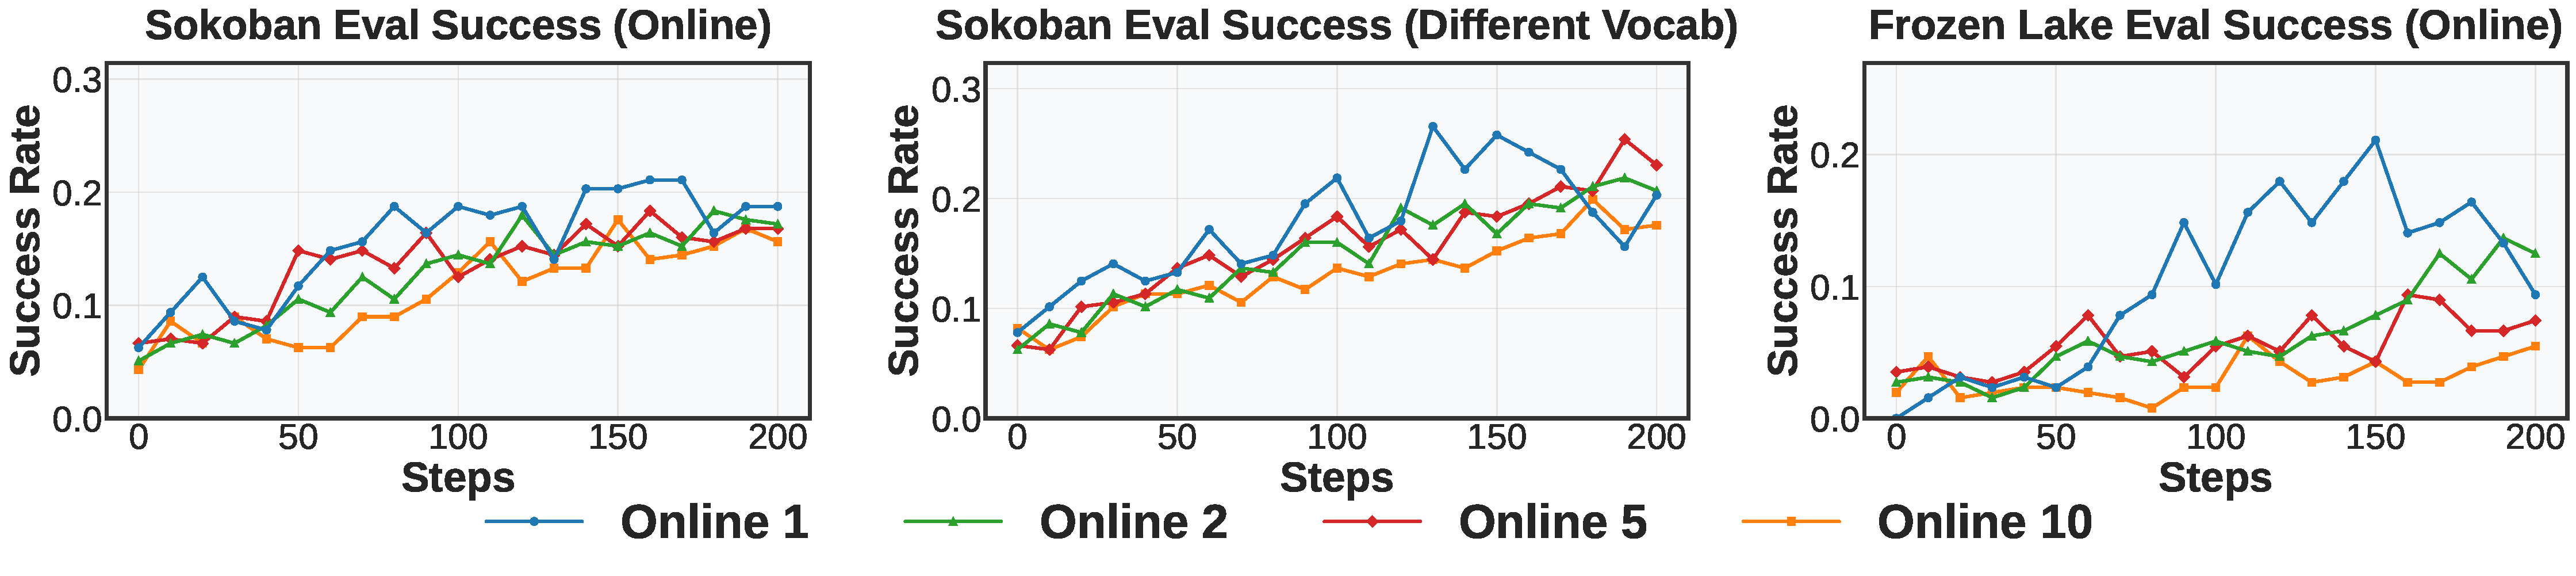
\includegraphics[width=\textwidth]{figures/figures_combined/figure_10_rollout_effect.pdf}
\caption{\textbf{Performance under different rollout frequencies (\textit{Online-\(k\)}).} We vary the rollout reuse factor \(k\), where each batch is reused for \(k\) policy updates. Lower \(k\) (e.g., \textit{Online-1}) means more frequent rollouts. Fresher data improves convergence by staying aligned with the current policy.} 
  \label{fig:rollout_freq}
\vspace{-15pt}
\end{figure}





\begin{onebox}{Finding 6: Reasoning fails to emerge without meticulous reward design}
While symbolic reasoning can emerge in simple, single-turn tasks under weak supervision, it fails to persist in multi-turn environments without the reward design explicitly encouraging interpretable intermediate reasoning steps. We observe that even with structured prompts, reasoning gradually decays during training if the reward signal focuses only on final outcomes. This suggests that without meticulous reward shaping, agents may tend to collapse into shortcut behaviors that bypass reasoning altogether.
\end{onebox}

